\section{Parcelamiento del hemisferio izquierdo}

Estos son los resultados de parcelar el hemisferio izquierdo con un total de
aproximadamente $24000$ semillas. 

\subsection{M\'etodo Moreno-Dominguez}

Las figuras \ref{fig:moreno_corteza0}; \ref{fig:moreno_corteza1} y \ref{fig:moreno_corteza2}
muestran las parcelas obtenidas usando $k=10000$ a distintos niveles de profundidad
del dendrogama.

\begin{figure}[h!]
    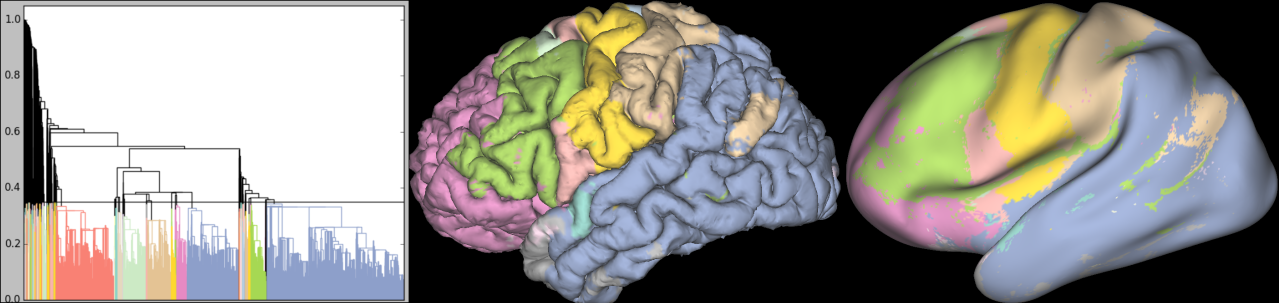
\includegraphics[width=\textwidth]{img/all_brain/moreno_10000.png}
    \caption{M\'etodo Moreno-Dominguez, primeras 10000 uniones entre vecinos}
    \label{fig:moreno_corteza0}
\end{figure}

\begin{figure}[h!]
    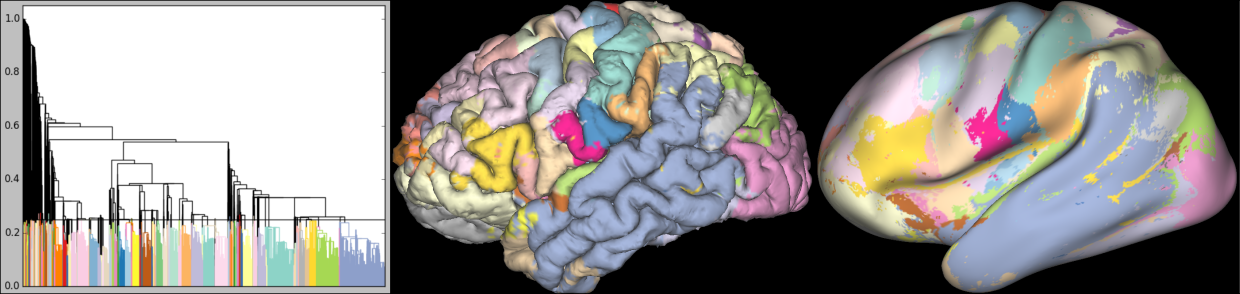
\includegraphics[width=\textwidth]{img/all_brain/moreno_10000_deep0.png}
    \caption{M\'etodo Moreno-Dominguez, primeras 10000 uniones entre vecinos, mayor profundidad}
    \label{fig:moreno_corteza1}
\end{figure}

\begin{figure}[h!]
    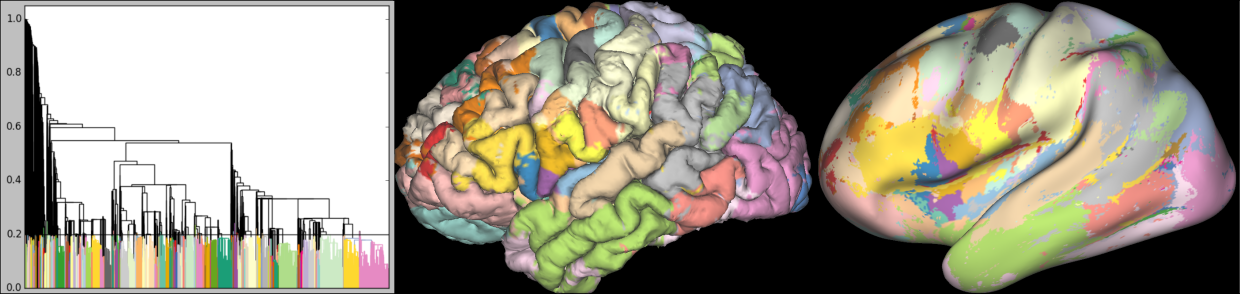
\includegraphics[width=\textwidth]{img/all_brain/moreno_10000_deep1.png}
    \caption{M\'etodo Moreno-Dominguez, primeras 10000 uniones entre vecinos, mayor profundidad}
    \label{fig:moreno_corteza2}             
\end{figure}

\clearpage

\subsection{Utilizando nuestro m\'etodo}

Las figuras \ref{fig:nosotros_corteza0} y \ref{fig:nosotros_corteza1} muestran 
las parcelas obtenidas usando $k=0$ a distintos niveles de profundidad del dendrogama.
Las figuras \ref{fig:nosotros_corteza2}; \ref{fig:nosotros_corteza3} y
\ref{fig:nosotros_corteza4} muestran los resultados usando $k=20000$  a distintos
niveles de profundidad del dendrograma.

\begin{figure}[h!]
    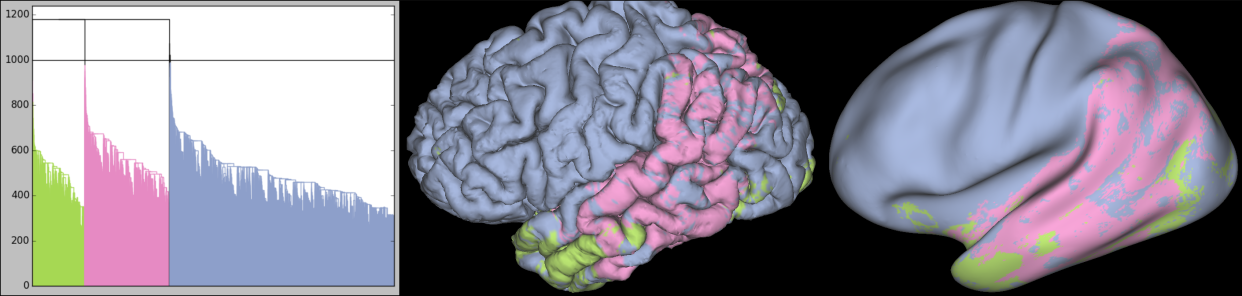
\includegraphics[width=\textwidth]{img/all_brain/logit_0.png}
    \caption{Nuestro m\'etodo sin restricciones}
    \label{fig:nosotros_corteza0}
\end{figure}
                                                                                                                        
\begin{figure}[h!]
    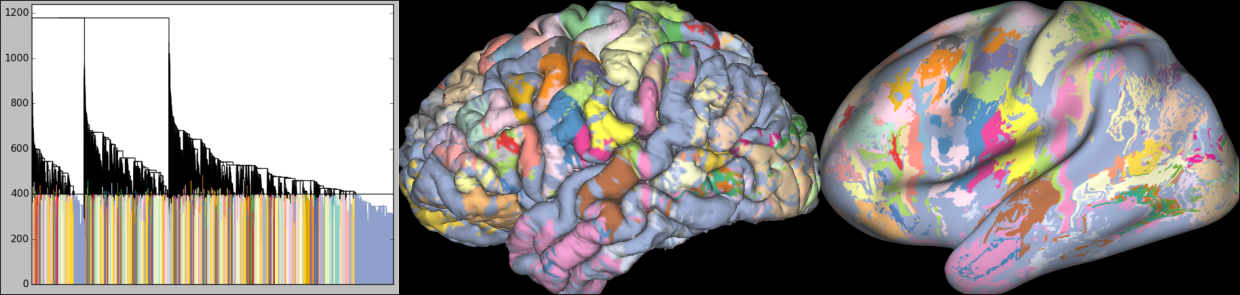
\includegraphics[width=\textwidth]{img/all_brain/logit_0_deep.png}
    \caption{Nuestro m\'etodo sin restricciones, mayor profundidad en el 
            dendrograma}
    \label{fig:nosotros_corteza1}
\end{figure}

\begin{figure}[h!]
    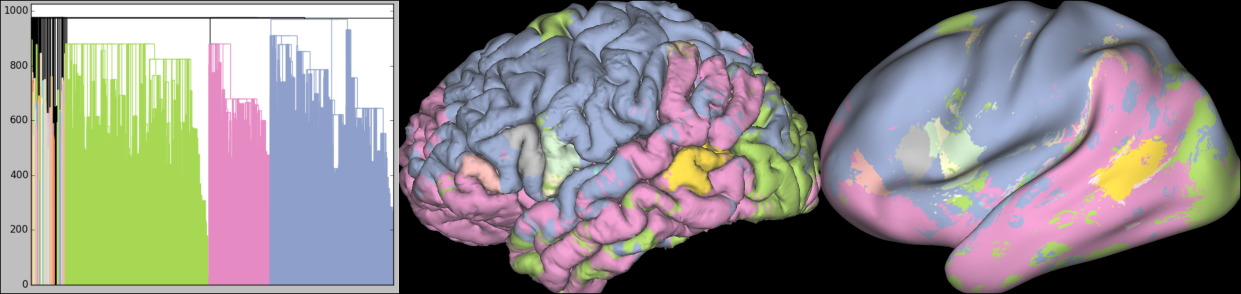
\includegraphics[width=\textwidth]{img/all_brain/logit_20000.png}
    \caption{Nuestro m\'etodo, primeras 20000 uniones entre vecinos}
    \label{fig:nosotros_corteza2}
\end{figure}

\begin{figure}[h!]
    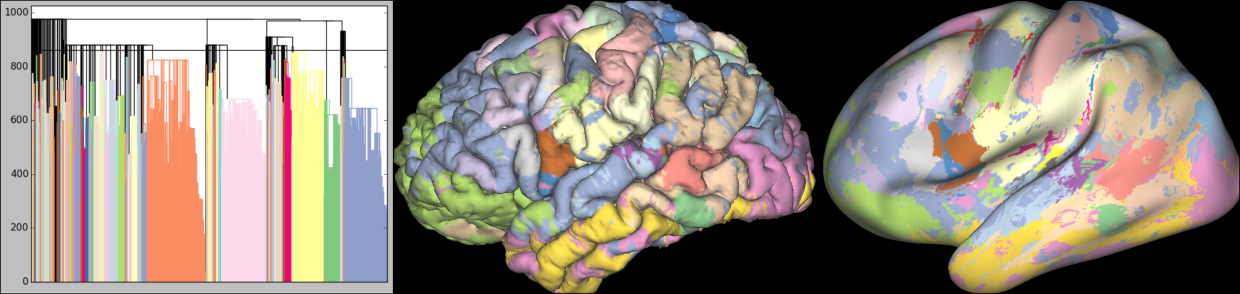
\includegraphics[width=\textwidth]{img/all_brain/logit_20000_deep0.png}
    \caption{Nuestro m\'etodo, primeras 20000 uniones entre vecinos, mayor profundidad}
    \label{fig:nosotros_corteza3}
\end{figure}

\begin{figure}[h!]
    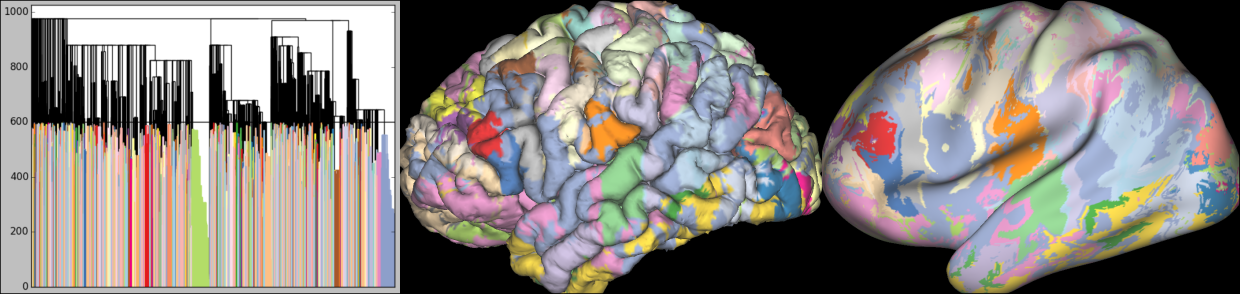
\includegraphics[width=\textwidth]{img/all_brain/logit_20000_deep1.png}
    \caption{Nuestro m\'etodo, primeras 20000 uniones entre vecinos, mayor profundidad}
    \label{fig:nosotros_corteza4}
\end{figure}

\subsection{Acercamiento a ambos m\'etodos}
\label{sec:acercamiento_corteza}

La figura \ref{fig:vs_moreno} presenta la corteza parcelada usando el m\'etodo 
Moreno-Dominguez con $k=10000$. La figura \ref{fig:vs_nosotros} muestra el 
resultado de usar nuestro m\'etodo con $k=20000$.

\begin{figure}[h!]
    \centering
    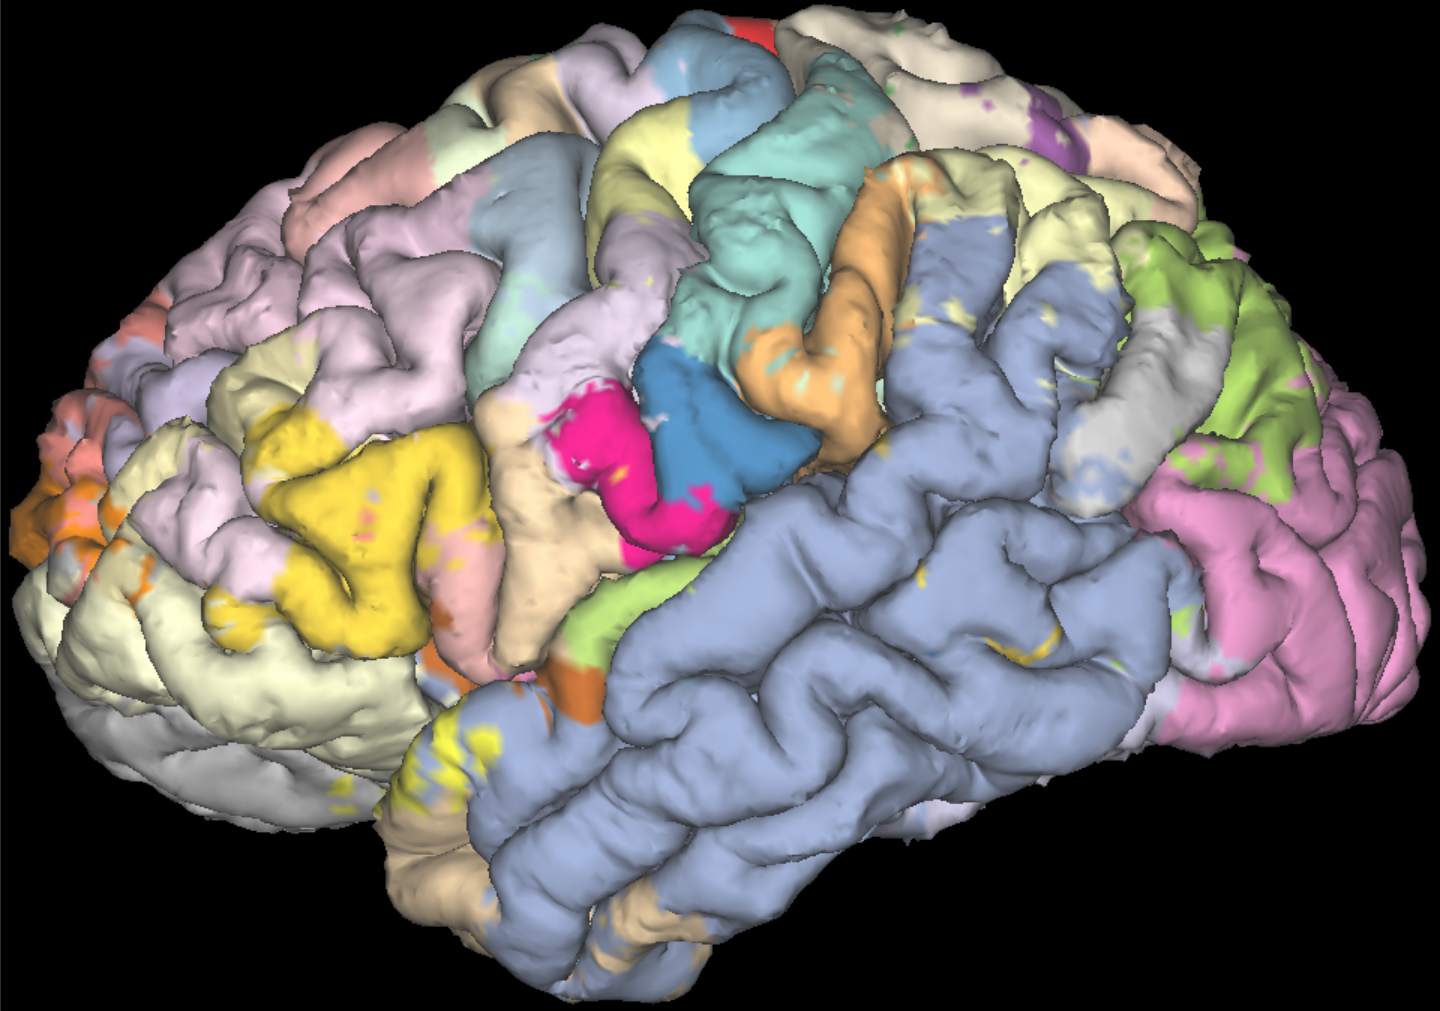
\includegraphics[width=0.62\textwidth]{img/all_brain/vs_moreno.png}
    \caption{M\'etodo Moreno-Dominguez, primeras 10000 uniones entre vecinos}
    \label{fig:vs_moreno}
\end{figure}

\begin{figure}[h!]
    \centering
    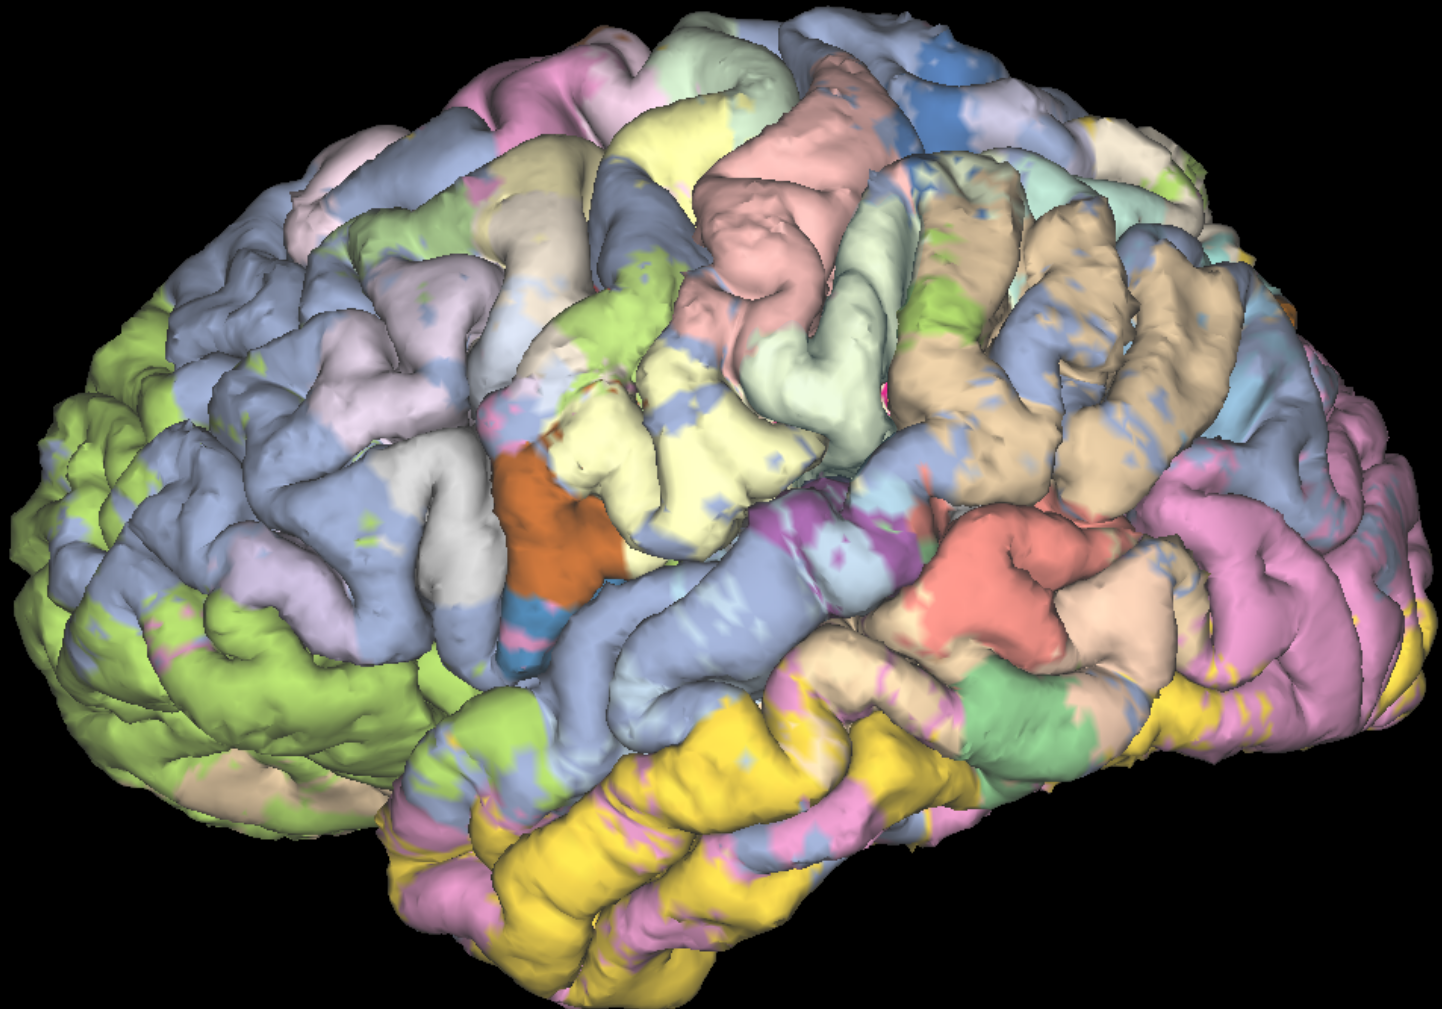
\includegraphics[width=0.62\textwidth]{img/all_brain/vs_nuestro.png}
    \caption{Nuestro m\'etodo, primeras 20000 uniones entre vecinos}
    \label{fig:vs_nosotros}
\end{figure}


